\chapter{Eclipse als Java-Entwicklungsumgebung}
\newcommand{\chaptertitle}{Eclipse als Java-Entwicklungsumgebung}

\lehead[]{\normalfont\sffamily\hspace*{-2.00cm}\textcolor{white}{\colorbox{lightblue}{\makebox[1.60cm][r]{\thechapter}}}\hspace{0.17cm}\textcolor{lightblue}{\chaptertitle}}
\rohead[]{\textcolor{lightblue}{\chaptertitle}\normalfont\sffamily\hspace*{0.17cm}\textcolor{white}{\colorbox{lightblue}{\makebox[1.60cm][l]{\thechapter}}}\hspace{-2.00cm}}
%\chead[]{}
\rehead[]{\textcolor{lightblue}{AvHG, Inf, My}}
\lohead[]{\textcolor{lightblue}{AvHG, Inf, My}}


\section{Vorbereitung}

%\subsection{Installation des Java-SDKs}
%
%Installiere das aktuelle JDK auf deinem Computer:
%
%\url{http://www.oracle.com/technetwork/java/javase/downloads/index.html}
%
%$\rightarrow$ \myPMI{JDK} $\rightarrow$ \myPMI{Download} $\rightarrow$
%\myPMI{Accept License Agreement}
%
%Aus der Liste wählst du die für dein Betriebssystem und Architektur (32bit oder
%64bit) passende Datei aus.

\subsection{Anlegen eines Git-Repositories für deine Java-Dateien}

Spätestens wenn mehrere Personen (oft dazu noch an unterschiedlichen Orten)
gemeinsam an einem Software-Projekt arbeiten, macht es keinen Sinn mehr seine
Programm-Quelltexte auf der lokalen Festplatte zu speichern. Vielmehr werden
dann Versionsverwaltungssysteme – sogenannte Repositories –  benutzt, 
die die Daten online an einer zentralen Stelle bereit halten. Siehe

\url{http://de.wikipedia.org/wiki/Repository}

\subsubsection{Git}

Git ist ein modernes System zur verteilten Versionsverwaltung. Es wurde 2005 von
Linus Torvalds, dem Erfinder von Linux, als Open Source Alternative zum bis
dahin für die Linux Kernel Entwicklung eingesetzten BitKeeper System entwickelt.

Die Versionsverwaltung mit Git erfolgt zunächst einmal in einem Verzeichnis auf
dem lokalen Rechner. Üblicherweise wird man irgendwo im Internet einen
Git-Server benutzen, der als zentrales Repository dient, über den der Austausch
zwischen beliebig vielen lokalen Repositories (für uns: typischerweise eines zu
Hause und eines in der Schule) läuft.

Es gibt mehrere Anbieter von kostenlosen Git-Servern. Der bekannteste ist
wohl Github. Bei einem anderen Provider, nämlich GitLab, kann man nicht nur
öffentliche, sondern auch private (also für andere nicht einsehbare) kostenlos Repositories
anlegen:

\url{https://gitlab.com/users/sign_in}

Dazu musst du dich mit einer gültigen e-Mail Adresse registrieren (siehe
Abbildung \ref{fig:gitlab-account-creation}).

\begin{figure}[h]
  \centering
   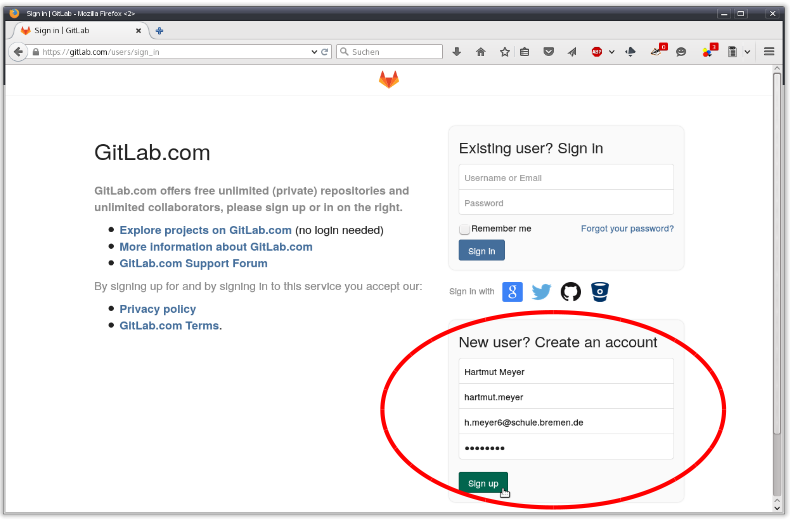
\includegraphics[width=1.0\textwidth]{./inf/SEKII/01_Vorbereitung/GitLab_Account_Creation.png}
   \caption{Anlegen eines Accounts bei gitlab.com}
   \label{fig:gitlab-account-creation}
\end{figure}

Du kannst Eclipse auch ohne solch ein Git-Repository nutzen, oder ein
kostenloses Repositories eines anderen Providers nutzen.

Am Beispiel von GitLab wird jetzt gezeigt, wie du dir ein eigenes Projekt
anlegst. Bei anderen Providern würde es ganz ähnlich funktionieren.

Nach der erfolgreichen Registrierung bei GitLab hast du dort ein Benutzerkonto,
aber noch keine Projekte. Nach der Anmeldung findest du direkt auf der
Startseite einen Button, um ein neues Projekt anzulegen (Abbildung
\ref{fig:gitlab-new-project-1}).

\begin{figure}[h]
  \centering
   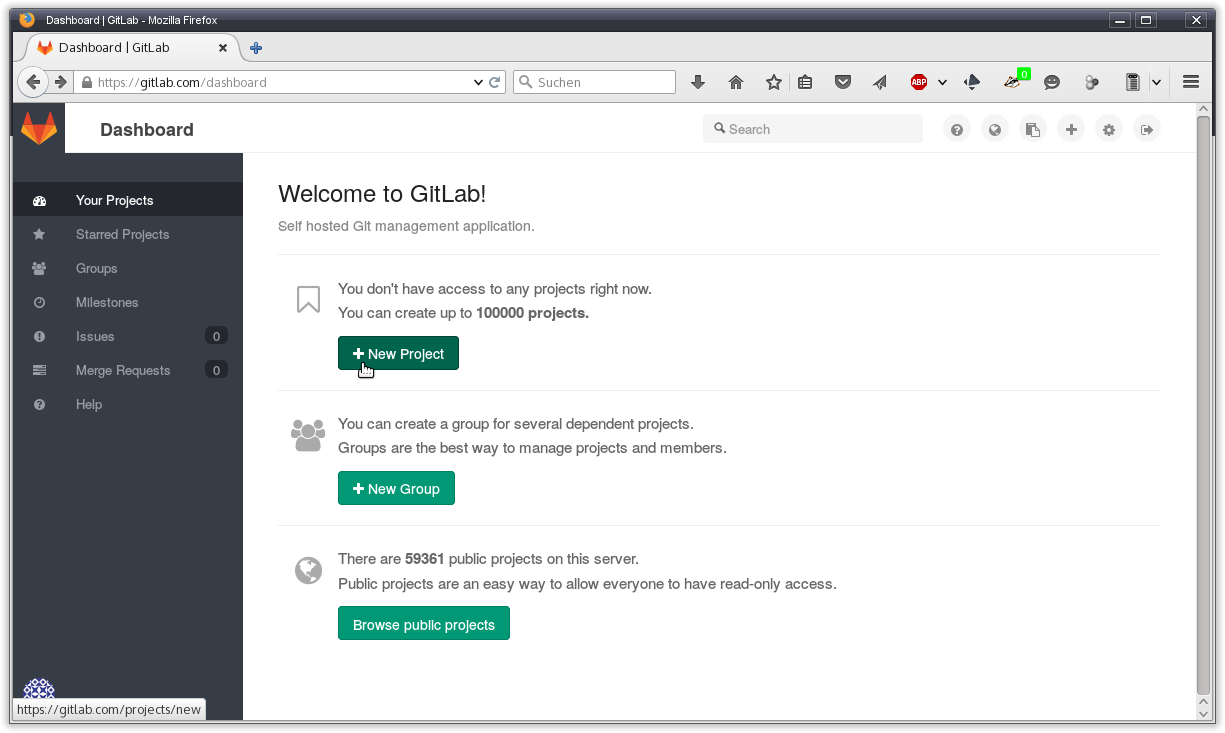
\includegraphics[width=1.0\textwidth]{./inf/SEKII/01_Vorbereitung/GitLab_New_Project_1.png}
   \caption{Anlegen eines eigenen Projects bei GitLab (1)}
   \label{fig:gitlab-new-project-1}
\end{figure}

Auf der folgenden Seite musst du einen Namen für dein Projekt wählen (Abbildung
\ref{fig:gitlab-new-project-2}).

\begin{figure}[h]
  \centering
   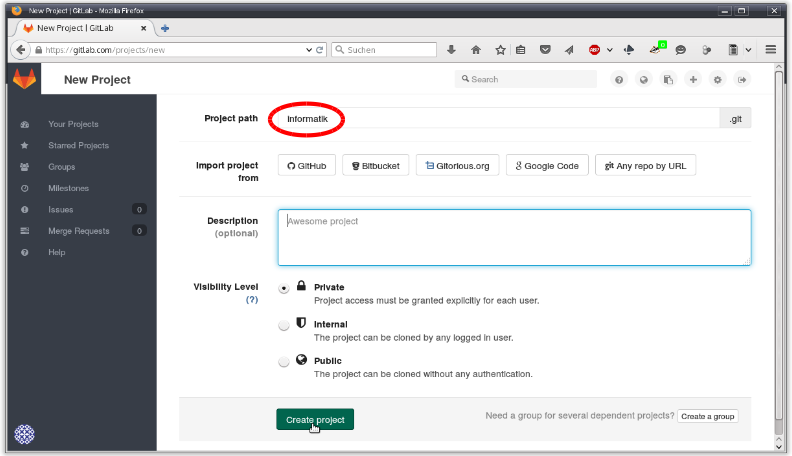
\includegraphics[width=1.0\textwidth]{./inf/SEKII/01_Vorbereitung/GitLab_New_Project_2.png}
   \caption{Anlegen eines eigenen Projects bei GitLab (2)}
   \label{fig:gitlab-new-project-2}
\end{figure}

Im letzten Schritt solltest du dir die Adresse (URL) deines Repositories
notieren. Dazu musst du zunächst auf den Button \myPMI{HTTPS} klicken. Außerdem
solltest du an dieser Stelle die angebotene Möglichkeit nutzen, eine README
Datei anzulegen. Erst mit dieser Readme Datei kann man das Repository
anschließend direkt nutzen! Siehe Abbildung \ref{fig:gitlab-new-project-3}.

\begin{figure}[h]
  \centering
   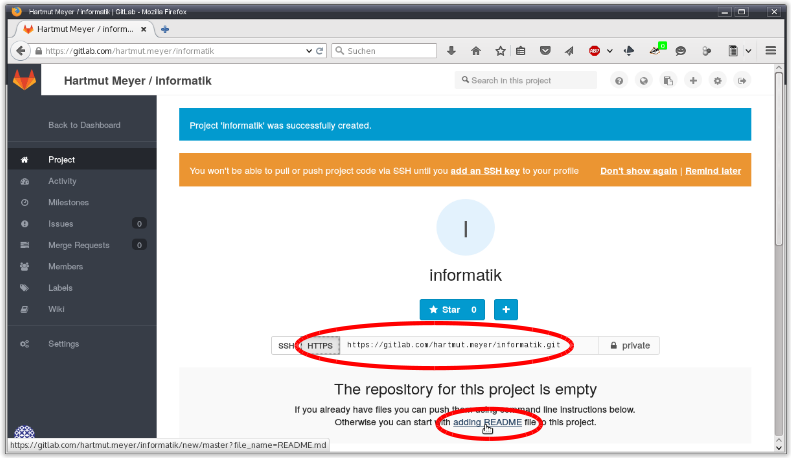
\includegraphics[width=1.0\textwidth]{./inf/SEKII/01_Vorbereitung/GitLab_New_Project_3.png}
   \caption{Anlegen eines eigenen Projects bei GitLab (3)}
   \label{fig:gitlab-new-project-3}
\end{figure}

Der Inhalt der README Datei ist völlig nebensächlich. Ein Punkt, oder irgendein
Nonsense. Aber eben mindestens ein Zeichen. Damit die neue Datei im
Repository angelegt werden kann, musst du auch eine sogenannte \emph{Commit
Message} schreiben. Erst danach ist der Button \myPMI{Commit Changes} aktiv.

Der Inhalt der Commit Message ist hier übrigens genauso egal wie der Inhalt der
README Datei.

Nach dem Commit ist dein eigenes Projekt angelegt, und du kannst es nun als
Git-Repository nutzen.




%\afterpage{\clearpage}

% \subsubsection{Subversion}
% 
% Statt Git könnten wir auch Subversion benutzen. Beim Anbieter assembla.com
% kannst du dir hier
% 
% \url{https://www.assembla.com/user/one_page_signup?space_type=public}
% 
% kostenlos ein öffentliches Subversion-Repository anlegen. Dazu musst du dich
% allerdings registrieren (siehe Abbildung \ref{fig:assembla-account-creation}).
% 
% \begin{figure}[h]
%   \centering
%    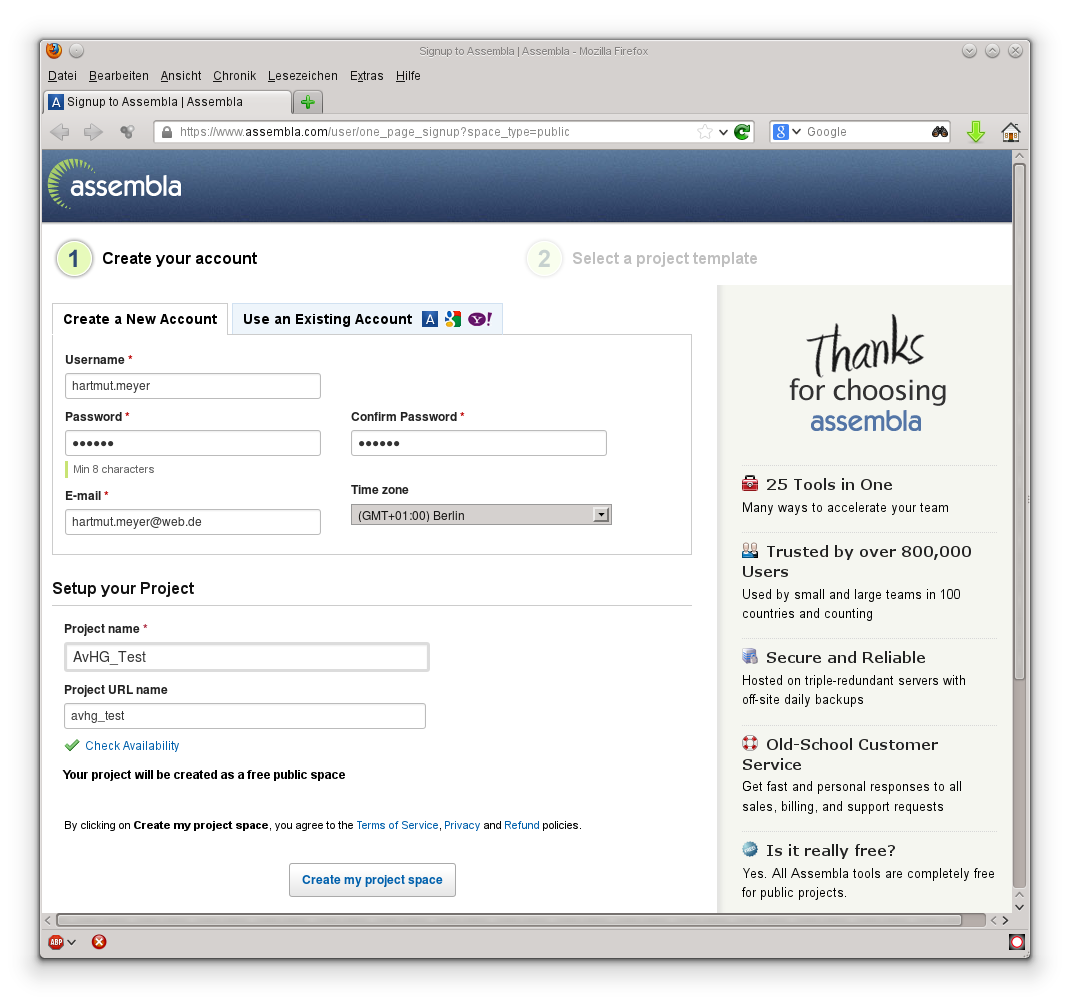
\includegraphics[width=1.0\textwidth]{./inf/SEKII/01_Vorbereitung/Assembla_Account_Creation.png}
%    \caption{Anlegen eines Accounts bei assembla.com}
%    \label{fig:assembla-account-creation}
% \end{figure}
% 
% Bei \myUserInput{Select a Project Configuration} (siehe Abbildung
% \ref{fig:assembla-project-configuration}) wählst du \myUserInput{Task and Issue
% Management with Integrated Subversion Hosting}.
% 
% \begin{figure}[h]
%   \centering
%    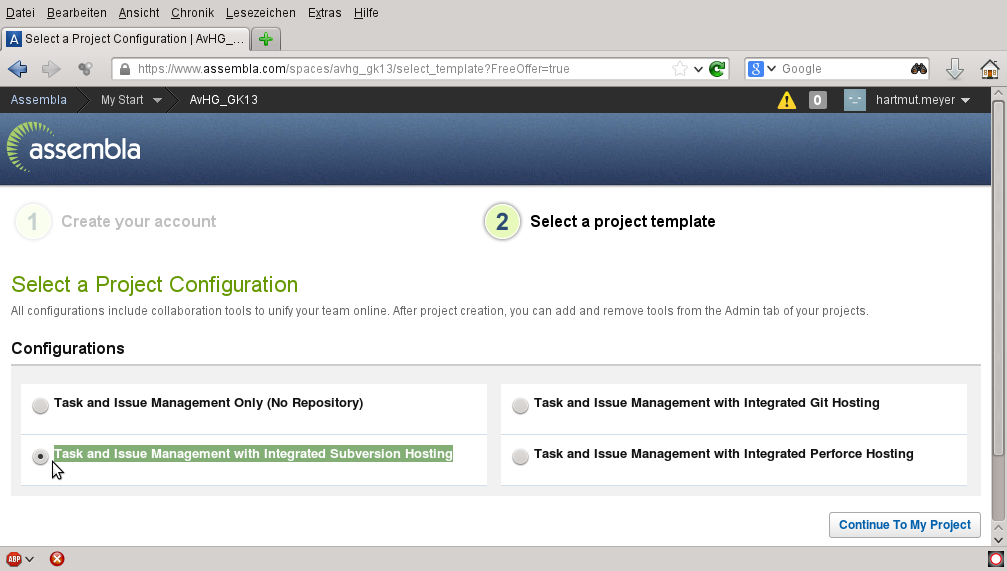
\includegraphics[width=1.0\textwidth]{./inf/SEKII/01_Vorbereitung/Assembla_Project_Configuration.png}
%    \caption{Projekt Konfiguration mit Subversion-Repository wählen}
%    \label{fig:assembla-project-configuration}
% \end{figure}
% 
% Du kannst Eclipse auch ohne solch ein Subversion-Repository nutzen, wenn dir
% das lieber ist.

\clearpage

\section{Eclipse herunterladen und installieren}

Die jeweils aktuellste stabile Version von Eclipse findest du hier:	

\url{https://www.eclipse.org/downloads/}

Dort wählst du den 64-Bit Download von Eclipse, passend für dein Betriebssystem.
Heruntergeladen wird so der Eclipse-Installer, den du anschließend startest.

Von den dort angebotenen Paketen solltest du \glqq Eclipse IDE for Java
Developers\grqq\ auswählen (Abbildung \ref{fig:eclipse-installer}). 

\begin{figure}[h]
  \centering
  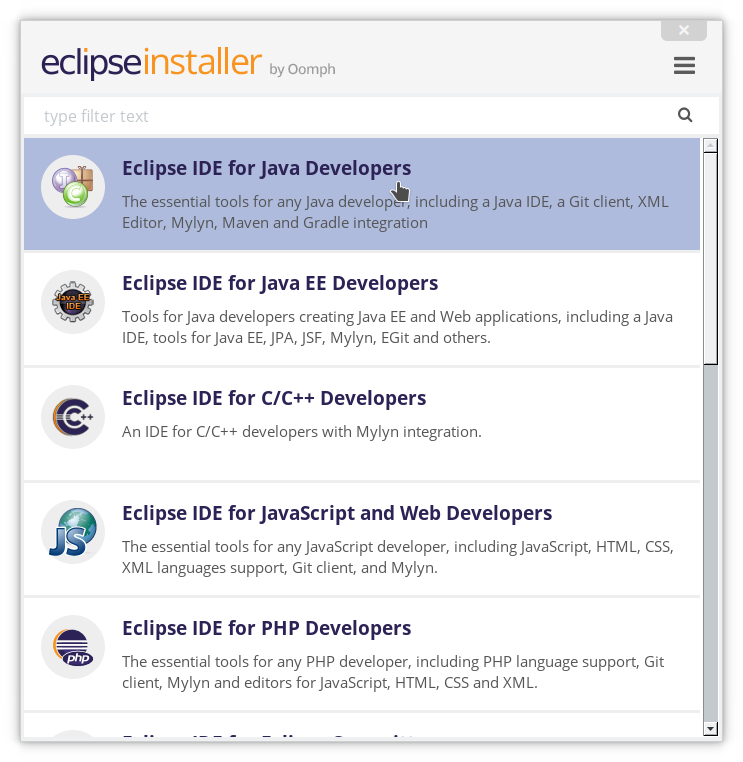
\includegraphics[width=0.7\textwidth]{./inf/SEKII/01_Vorbereitung/Eclipse-Installer.png}
  \caption{Preferences-Dialog für die Workspace-Einstellungen}
  \label{fig:eclipse-installer}
\end{figure}

Wenn du mit Windows arbeitest, wird dir zum Abschluss der Installation angeboten, eine Verknüpfung 
auf dem Desktop anzulegen und einen Eintrag im Startmenü zu erzeugen.


\section{Eclipse konfigurieren}

\subsection{Zeichensatz festlegen}

Damit ihr untereinander und mit mir problemlos Dateien austauschen könnt,
solltet ihr als erstes den Zeichensatz festlegen, mit dem Eclipse eure
Textdateien (also auch die Java-Quelltext Dateien) interpretiert. Dies ist im
Besonderen bedeutsam für die Kodierung von Umlauten und sonstigen
Sonderzeichen.

In Eclipse: \myPMI{Window} $\rightarrow$ \myPMI{Preferences} $\rightarrow$
\myPMI{General} $\rightarrow$ \myPMI{Workspace} $\rightarrow$ \myPMI{Text
file encoding} $\rightarrow$ \myPMI{Other} $\rightarrow$ \myPMI{UTF-8}

(Abbildung \ref{fig:eclipse-workspace-preferences}) 

\subsection{Änderungen durch andere Programme im Workspace überwachen}

Eclipse geht normalerweise davon aus, dass die Dateien im Eclipse-eigenen
Arbeitsverzeichnis (Workspace) nur aus Eclipse selbst heraus angelegt, gelöscht
oder verändert werden.

Das hat zur Folge, dass Eclipse durcheinander kommen kann, wenn du
beispielsweise mit einem externen Programm eine Datei im Workspace veränderst
oder Dateien dort hinein kopierst, löscht oder umbenennst.
Es ist aber leicht, Eclipse so einzustellen, dass externe Änderungen an Dateien
im Workspace erkannt werden:

\myPMI{Window} $\rightarrow$ \myPMI{Preferences} $\rightarrow$
\myPMI{General} $\rightarrow$ \myPMI{Workspace} $\rightarrow$
Häkchen setzen vor \myPMI{Refresh using native hooks or polling}.

(Abbildung \ref{fig:eclipse-workspace-preferences}) 

\begin{figure}[h]
  \centering
  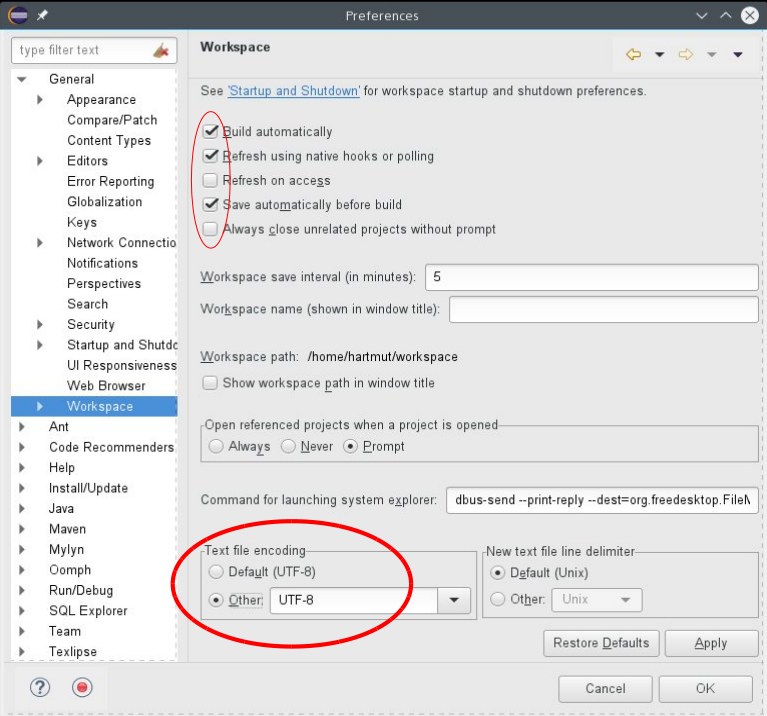
\includegraphics[width=0.83\textwidth]{./inf/SEKII/01_Vorbereitung/Eclipse-Workspace-Preferences.png}
  \caption{Preferences-Dialog für die Workspace-Einstellungen}
  \label{fig:eclipse-workspace-preferences}
\end{figure}

%\afterpage{\clearpage}

\subsection{Git-Funktionalität in Eclipse konfigurieren und dein eigenes
Repository einbinden}

%Im Preferences Dialog (\myPMI{Window} $\rightarrow$ \myPMI{Preferences}) sollte
%nun der Standard-Ort für die lokalen Git-Reposities (Abbildung
%\ref{fig:eclipse-git-configuration-1}) 
%sowie die e-Mail Adresse (Abbildung \ref{fig:eclipse-git-configuration-2})
%eingestellt werden.
%
%\begin{figure}[h]
%  \centering
% 
% 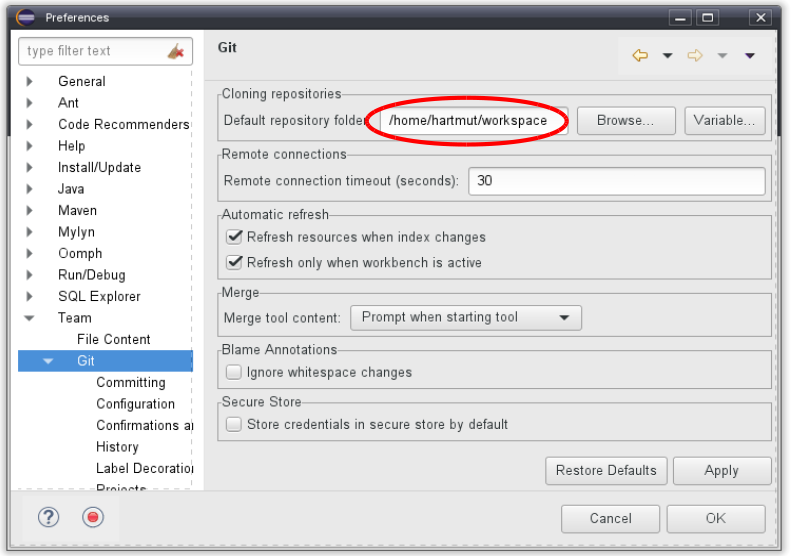
\includegraphics[width=0.84\textwidth]{./inf/SEKII/01_Vorbereitung/Eclipse-Git-Configuration-1.png} \caption{Standard-Verzeichnis für lokale Git-Repositories wählen (dort musst
%  du den Ort für \emph{dein} Workspace Verzeichnis angeben)}
%  \label{fig:eclipse-git-configuration-1}
%\end{figure}
%
%\begin{figure}[h]
%  \centering
%  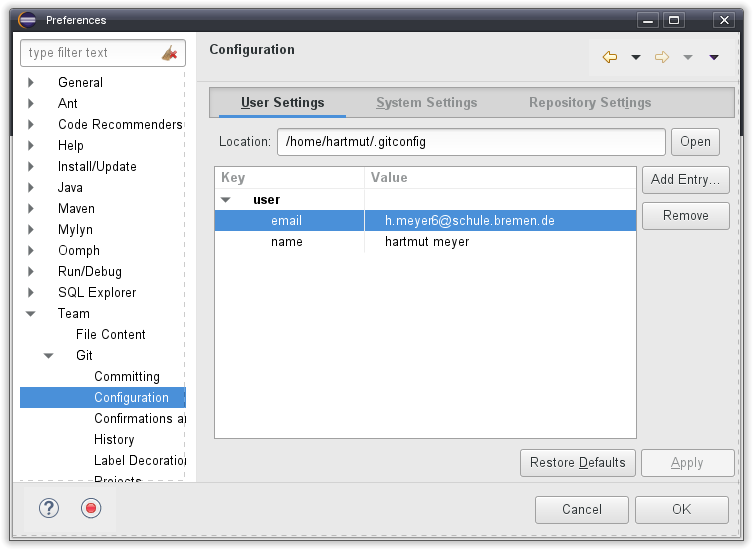
\includegraphics[width=0.85\textwidth]{./inf/SEKII/01_Vorbereitung/Eclipse-Git-Configuration-2.png}
%  \caption{e-Mail Adresse für Git-Commits wählen}
%  \label{fig:eclipse-git-configuration-2}
%\end{figure}
%
%\afterpage{\clearpage}
%
%Damit ist Eclipse grundsätzlich für die Arbeit mit Git-Repositories
% vorbereitet.
%
Um nun dein eigenes Repository in Eclipse nutzen zu können, musst du einige
wenige Konfigurationsschritte durchführen:

\subsubsection{Fall 1: Erstmaliges Einbinden eines zuvor beim Git-Hoster
angelegten Repositories (machst du typischerweise in der Schule)}

Wenn du bisher noch kein eigenes Java-Projekt angelegt hast, dann bist du hier
richtig. Ansonsten folgst du bitte den Anweisungen im nächsten Abschnitt
(Fall 2).

\myPMI{File} $\rightarrow$ \myPMI{Import\ldots} $\rightarrow$ \myPMI{Git}
$\rightarrow$ \myPMI{Projects from Git} $\rightarrow$ \myPMI{Next} $\rightarrow$
\myPMI{Clone URI} $\rightarrow$ \myPMI{Next} Per Coyp \& Paste die URI
(https://gitlab.com/\ldots) einfügen sowie dein Benutzername und Passwort für
GitLab(!) (Abbildung \ref{fig:import-project-from-git})

\begin{figure}[h]
  \centering
   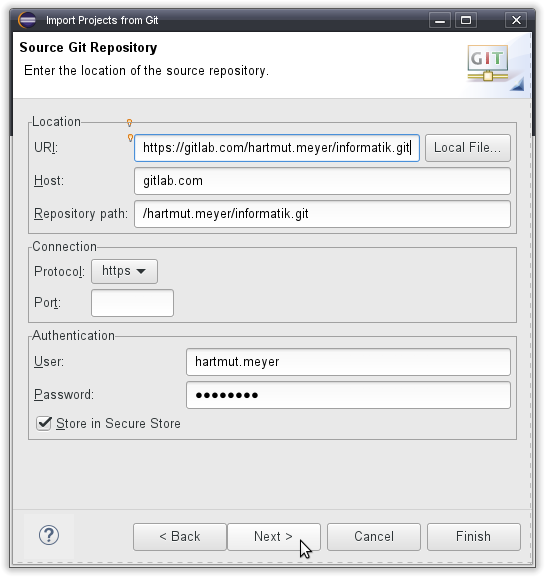
\includegraphics[width=0.70\textwidth]{./inf/SEKII/01_Vorbereitung/Import_Project_from_Git.png}
   \caption{Ein eigenes Java-Projekt in Eclipse anlegen (erster Schritt)}
   \label{fig:import-project-from-git}
\end{figure}

Von dort aus weiter: $\rightarrow$ \myPMI{Next} $\rightarrow$ \myPMI{Next}
$\rightarrow$ \myPMI{Next} 

(Abbildung \ref{fig:import-project-from-git-using-wizard-1})

$\rightarrow$ \myPMI{Finish} $\rightarrow$ \myPMI{Java} $\rightarrow$
\myPMI{Java Project}

(Abbildung \ref{fig:import-project-from-git-using-wizard-2})

$\rightarrow$ \myPMI{Next}  $\rightarrow$ Bei \myPMI{Project Name:} einen Namen
für dein Projekt wählen (kann, muss aber nicht identisch sein, mit dem Namen,
den du bei GitLab für dein Projekt gewählt hast) \myPMI{Next} $\rightarrow$
\myPMI{Finish}

\begin{figure}[h]
  \centering
   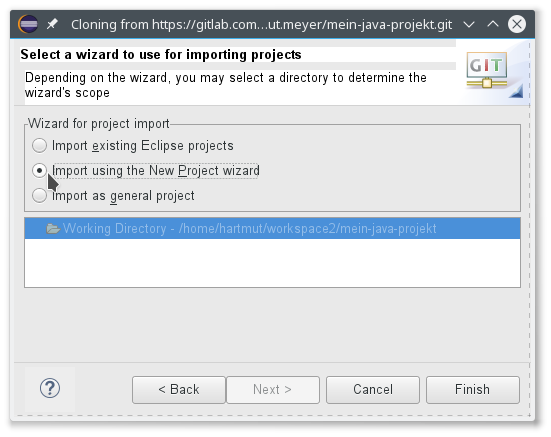
\includegraphics[width=0.70\textwidth]{./inf/SEKII/01_Vorbereitung/Import_Project_from_Git_using_Project_Wizard_1.png}
   \caption{Ein eigenes Java-Projekt in Eclipse anlegen (using Project Wizard)}
   \label{fig:import-project-from-git-using-wizard-1}
\end{figure}

\begin{figure}[h]
  \centering
   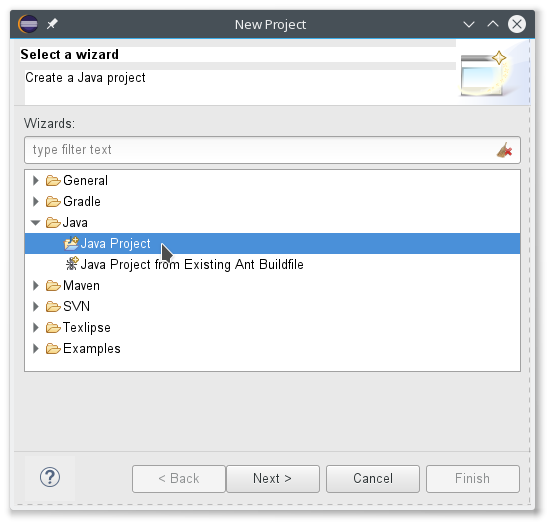
\includegraphics[width=0.70\textwidth]{./inf/SEKII/01_Vorbereitung/Import_Project_from_Git_using_Project_Wizard_2.png}
   \caption{Ein eigenes Java-Projekt in Eclipse anlegen (Project Wizard: Java Project)}
   \label{fig:import-project-from-git-using-wizard-2}
\end{figure}

%\afterpage{\clearpage}

\clearpage

Mit einem Rechts-Klick auf das neue Projekt (im Package-Explorer nun sichtbar)
wählst du \myPMI{New} $\rightarrow$ \myPMI{Package}. Paket-Namen sollten immer
mit einem kleinen Buchstaben beginnen. Indem du das Projekt „auffaltest“
(Projekt $\rightarrow$ src) siehst du die vorhandenen Pakete des Projektes. Ein
Rechts-Klick auf ein Paket und ein \myPMI{New} $\rightarrow$ \myPMI{Class}
erzeugt einen Dialog, in dem man den Namen der neuen Java-Klasse wählen kann.
Mit einem Rechts-Klick auf ein Projekt im Package-Explorer kann man das Projekt
auch in das zuvor angelegte Git-Repository schieben: \myPMI{Team}
$\rightarrow$ \myPMI{Commit} $\rightarrow$ Dort muss ein Kommentar
eingegeben werden, der den Commit beschreibt; Haken setzen um alle
neuen/geänderten Dateien im Projekt für den Commit zu markieren (Abbildung
\ref{fig:git-commit}) $\rightarrow$ \myPMI{Commit and Push}

Dieses Projekt ist nun im Repository angelegt und man kann ab sofort Dateien des
Projekts in dieses Repository sichern (\myPMI{Team} $\rightarrow$
\myPMI{Commit \ldots}) oder auch auf die Dateien aus dem Repository auf die
lokale Festplatte bringen (\myPMI{Team} $\rightarrow$ \myPMI{Pull})
-- etwa weil du zu Hause gearbeitet hast und nun in der Schule die Dateien auf
dem aktuellen Stand haben möchtest.

\subsubsection{Fall 2: Du hast dein eigenes Git-Repository bereits einmal in
Eclipse eingebunden und dort als Java-Projekt angelegt}

Wenn du dein eigenes Java-Projekt bereits einmal in dein damit
verknüpftes Git-Repository \glqq geschoben\grqq\ (\myPMI{Commit and Push}) hast,
aber es auf dem Computer an dem du gerade arbeitest (zum Beispiel zu Hause) noch
nicht in Eclipse eingebunden ist, dann kannst du es leicht aus deinem
Git-Repository importieren. Wichtig ist dabei, dass du dabei nicht noch einmal
den Projekt-Wizard von Eclipse benutzt, sondern einfach das bereits bestehende
Eclipse-Projekt aus dem Git-Repository importierst. 

\begin{figure}[h]
  \centering
   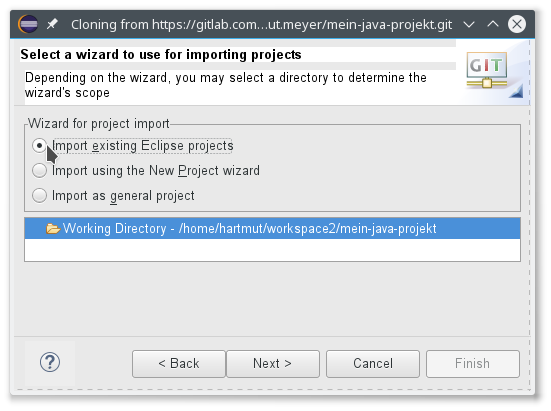
\includegraphics[width=0.70\textwidth]{./inf/SEKII/01_Vorbereitung/Import_Project_from_Git_Import_Existing_Eclipse_Project.png}
   \caption{Ein eigenes Java-Projekt in Eclipse anlegen (Import existing Eclipse projects)}
   \label{fig:import-project-from-git-import-existing-project}
\end{figure}

Abgesehen davon folgst du der Anleitung aus dem letzten Abschnitt (Fall 1).

Jetzt können lokale Änderungen in das Online-Repository geschrieben ("Commit
and Push") werden und umgekehrt das lokale Repository auf den Stand des
Online-Repositories gebracht werden ("Pull"):

\subsection{Git: Commit and Push}

Im Project Explorer: Rechtsklick auf eigenes Projekt $\rightarrow$ \myPMI{Team}
$\rightarrow$ \myPMI{Commit\ldots} $\rightarrow$ Dort muss ein Kommentar
eingegeben werden, der den Commit beschreibt; Haken setzen um alle
neuen/geänderten Dateien im Projekt für den Commit zu markieren (Abbildung
\ref{fig:git-commit}) $\rightarrow$ \myPMI{Commit and Push}

\begin{figure}[h]
  \centering
   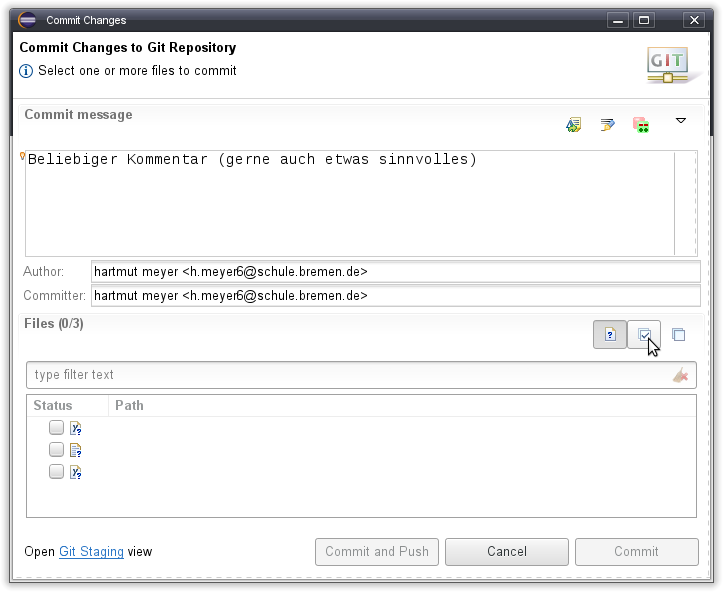
\includegraphics[width=0.85\textwidth]{./inf/SEKII/01_Vorbereitung/Git-Commit.png}
   \caption{Commit: Geänderte/neue Dateien in das Online-Repository schreiben}
   \label{fig:git-commit}
\end{figure}

\begin{figure}[h]
  \centering
   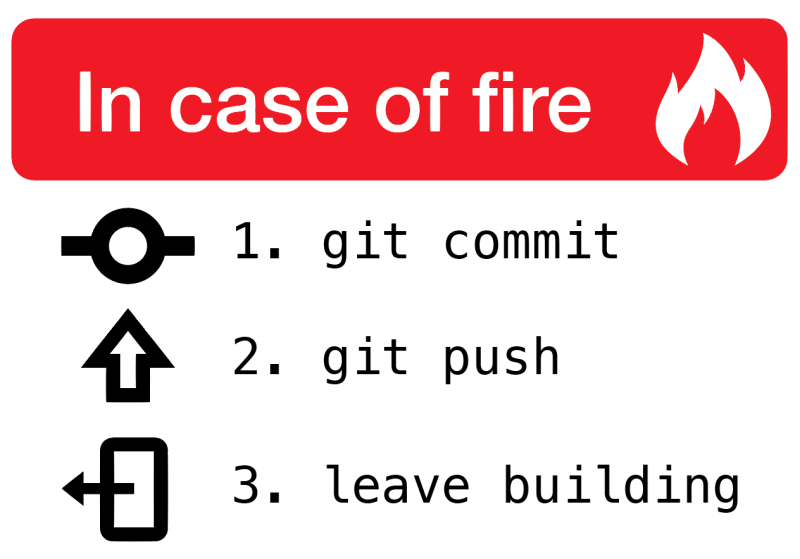
\includegraphics[width=0.35\textwidth]{./inf/SEKII/01_Vorbereitung/in-case-of-fire-1-git-commit-2-git-push-3-leave-building2.png}
   % https://hikaruzone.wordpress.com/2015/10/06/in-case-of-fire-1-git-commit-2-git-push-3-leave-building/
   % http://creativecommons.org/licenses/by-nc/4.0/
\end{figure}

\subsection{Git: Pull}

Im Project Explorer: Rechtsklick auf eigenes Projekt $\rightarrow$ \myPMI{Team}
$\rightarrow$ \myPMI{Pull}

\clearpage


% \subsection{Subversion Plugin „Subclipse“ installieren und dein eigenes
% Repository einbinden} 
% 
% Als nächstes solltest du noch eine Erweiterung zu Eclipse installieren um später
% mit deinem Sub\-vers\-ion-Repository arbeiten zu können. In Eclipse:
% \myPMI{Help} $\rightarrow$ \myPMI{Eclipse Marketplace \ldots} $\rightarrow$ In
% das Feld \myPMI{Find:} \myUserInput{subclipse} eintragen und mit \myPMI{Go}
% bestätigen. In der Trefferliste (nach kurzer Suche) hinter \myPMI{Subclipse}
% auf \myPMI{Install} klicken $\rightarrow$ \myPMI{Next} $\rightarrow$
% \myPMI{Next} $\rightarrow$ \myPMI{Accept License Agreement} $\rightarrow$
% \myPMI{Finish}.
% 
% Damit wird das Subclipse-Plugin installiert. Nach einem anschließend nötigen
% Neustart von Eclipse fügst du über \myPMI{Window} $\rightarrow$ \myPMI{Show
% View} $\rightarrow$ \myPMI{Other \ldots} $\rightarrow$ \myPMI{SVN}
% $\rightarrow$ \myPMI{SVN Repositories} den „SVN Repositories“-View hinzu
% (erscheint als zusätzlicher Reiter in dem Teilfenster unten). Ein Rechts-Klick
% in diesen View öffnet das dazu gehörige Kontext-Menü. Dort wählst du
% \myPMI{New} $\rightarrow$ \myPMI{Repository Location \ldots}. In dem Dialog
% gibst du dann als URL \url{https://subversion.assembla.com/svn/DEIN_REPOSITORY}
% an (den Namen deines Repositories hast du vorher bei der Registrierung bei
% assembla.com selber ausgewählt).
% 
% Um mit Eclipse arbeiten zu können musst du zu aller erst ein „Projekt“ anlegen.
% Dazu im linken Teil-Fenster (dem sogenannten „Package-Explorer“) ein
% Rechts-Klick und dann im Kontext-Menü \myPMI{New} $\rightarrow$ \myPMI{Java
% Project} auswählen. Nach der Wahl des Projekt-Namens kann direkt auf
% \myPMI{Finish} geklickt werden. 

% Mit einem Rechts-Klick auf das neue Projekt (im Package-Explorer nun sichtbar)
% wählst du \myPMI{New} $\rightarrow$ \myPMI{Package}. Paket-Namen sollten immer
% mit einem kleinen Buchstaben beginnen. Indem du das Projekt „auffaltest“
% (Projekt $\rightarrow$ src) siehst du die vorhandenen Pakete des Projektes. Ein
% Rechts-Klick auf ein Paket und ein \myPMI{New} $\rightarrow$ \myPMI{Class}
% erzeugt einen Dialog, in dem man den Namen der neuen Java-Klasse wählen kann.
% Mit einem Rechts-Klick auf ein Projekt im Package-Explorer kann man das Projekt
% auch in das zuvor angelegte Subversion-Repository schieben: \myPMI{Team}
% $\rightarrow$ \myPMI{Share Project \ldots} $\rightarrow$ \myPMI{SVN}
% $\rightarrow$ \myPMI{Next} $\rightarrow$ \myPMI{Next} $\rightarrow$
% \myPMI{Finish}. Dies muss nur ein mal für ein Projekt getan werden! 
% 
% Dieses Projekt ist nun im Repository angelegt und man kann ab sofort Dateien des
% Projekts in dieses Repository sichern (\myPMI{Team} $\rightarrow$
% \myPMI{Commit \ldots}) oder auch auf die Dateien aus dem Repository auf die
% lokale Festplatte bringen (\myPMI{Team} $\rightarrow$ \myPMI{Update to HEAD})
% -- etwa weil du zu Hause gearbeitet hast und nun in der Schule die Dateien auf
% dem aktuellen Stand haben möchtest.

\subsection{Das Kurs-Repository einbinden}

% \subsubsection{Git}

Alle Arbeitsblätter und sonstige Dateien werden euch über ein Kurs-Repository
zur Verfügung gestellt. Um auf dieses Kurs-Repository zugreifen zu können,
kannst du im Git Repositories View ein existierendes Git-Repository zu
\emph{clonen} (diese Möglichkeit wird über ein recht unscheinbares kleines Icon
am oberen rechten Rand des Git Repositories View angeboten: siehe Abbildung
\ref{fig:git-clone}).

\begin{figure}[h]
  \centering
   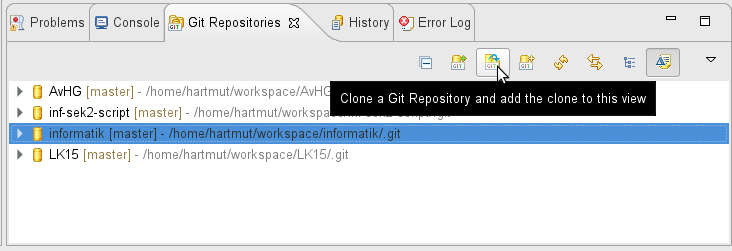
\includegraphics[width=0.8\textwidth]{./inf/SEKII/01_Vorbereitung/Cloning_a_Git_Repository.png}
   \caption{Commit: Ein existierendes Git-Repository clonen}
   \label{fig:git-clone}
\end{figure}

Dort gibst du im Feld \myPMI{URI}, die URL für euer Kurs-Repository ein. Etwa
\url{https://github.com/hartmutmeyer/LK15.git} an (der genaue Name eures
Kursverzeichnisses wird dir von mir mitgeteilt). Im dem folgenden Dialog
\myPMI{Clone Git Repository: Local Destination}, wählst du als Ordner deinen
Eclipse workspace aus. Dieser wird dann automatisch um den Namen des
Repositories ergänst.

Wenn du das Häkchen bei \myPMI{Import all existing Eclipse projects after clone
finishes} gesetzt lässt, wird nach Abschluss des Dialogs (und ggf.\ einer mehr
oder weniger langen Wartezeit, während derer die Dateien aus dem
Online-Repository auf die lokale Festplatte kopiert werden), im Projekt Explorer
neben deinem eigenen Repository auch das Kurs-Repository erscheinen.

Wichtig: Im Kurs-Repository hast du nur Lese-, aber keine Schreibrechte.
Folglich kannst du lokale Änderungen auch nicht mit einem Commit in das
Repository sichern. Wenn du Dateien aus dem Kurs-Repository ändern willst musst
du diese deshalb immer zuerst in dein eigenes Repository kopieren. Dort kannst
du sie dann bearbeiten und auch verändert mit einem Commit in dein eigenes
Repository sichern. Falls du versehentlich doch mal etwas im Kurs-Repository
verändert haben solltest (erkennbar am schwarzen Stern vor dem Ordner), dann
kannst du diese Änderungen ganz einfach mit Rechtsklick auf den
Ordner $\rightarrow$ \myPMI{Team} $\rightarrow$ \myPMI{Replace With}
$\rightarrow$ \myPMI{Branch, Tag, or Reference\ldots} $\rightarrow$
Doppelklick auf \myPMI{Remote Tracking} $\rightarrow$ \myPMI{origin/master}
$\rightarrow$ \myPMI{Replace} rückgängig machen.


% \subsubsection{Subversion}
% 
% Alle Arbeitsblätter und sonstige Dateien werden euch über ein Kurs-Repository
% zur Verfügung gestellt. Um auf dieses Kurs-Repository zugreifen zu können,
% fügst du mit Rechts-Klick im SVN Repository View das Kontext-Menü. Dort wählst
% du \myPMI{New} $\rightarrow$ \myPMI{Repository Location \ldots}. In dem Dialog
% gibst du dann als URL \url{https://subversion.assembla.com/svn/avhg_lk13} an
% (der genaue Name eures Kursverzeichnisses wird dir von mir mitgeteilt).
% 
% Im Repository View sollte nun nach kurzer Zeit neben deinem eigenen Repository
% auch die URL des Kurs-Repositories zu sehen sein. Dieses solltest du
% „aufklappen“ (Klick auf den Pfeil vor der URL).
% 
% \begin{figure}[h]
%   \centering
%    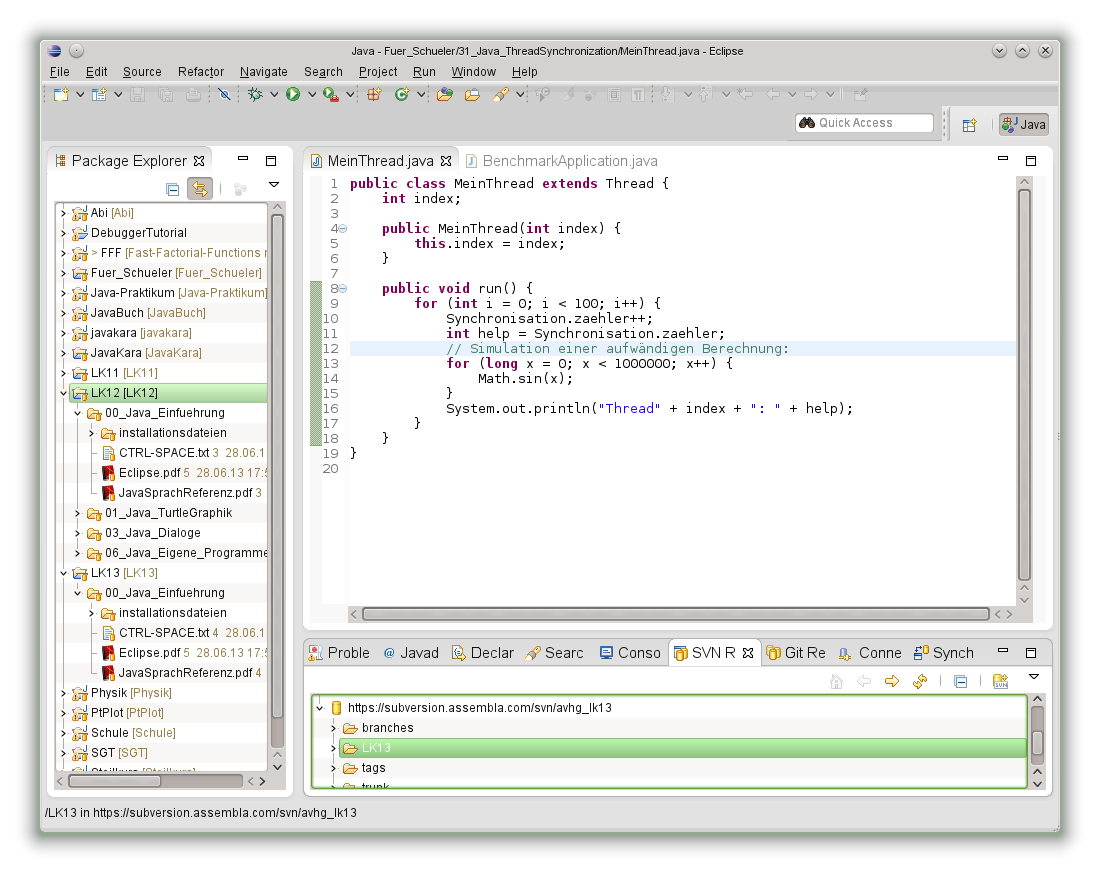
\includegraphics[width=1.0\textwidth]{./inf/SEKII/01_Vorbereitung/Eclipse_Repository-View.png}
%    \caption{Der SVN Repository View in Eclipse}
%    \label{fig:eclipse-repository-view}
% \end{figure}
% 
% Anschließend werden mehrere Ordner sichtbar (siehe Abbildung
% \ref{fig:eclipse-repository-view}). Mit Rechtsklick auf den Ordner \myFile{LK13}
% (bzw. den für euch passenden) bekommst du ein Kontext-Menü. Aus diesem wählst du
% den Eintrag \myPMI{Checkout \ldots}. Die folgende Dialog Box kannst direkt mit
% \myPMI{Finish} abschließen. Es dauert dann einige Zeit bis das Projekt aus dem
% Repository kopiert im Package-Explorer als eigenes Projekt auftaucht.
% 
% Wichtig: Im Kurs-Repository hast du nur Lese-, aber keine Schreibrechte.
% Folglich kannst du lokale Änderungen auch nicht mit einem Commit in das
% Repository sichern. Wenn du Dateien aus dem Kurs-Repository ändern willst musst
% du diese deshalb immer zuerst in dein eigenes Repository kopieren. Dort kannst
% du sie dann bearbeiten und auch verändert mit einem Commit in dein eigenes
% Repository sichern. Falls du versehentlich doch mal etwas im Kurs-Repository
% verändert haben solltest (erkennbar am schwarzen Stern vor dem Ordner), dann
% kannst du diese Änderungen ganz einfach mit Rechtsklick auf den
% Ordner $\rightarrow$ \myPMI{Team} $\rightarrow$ \myPMI{Revert\ldots} rückgängig
% machen.


\subsection{Zeilennummern anzeigen lassen}

Beim Programmieren ist es hilfreich, sich im Editor die Zeilennummern anzeigen
zu lassen. Dies stellst du wie folgt ein:

\myPMI{Window} $\rightarrow$ \myPMI{Preferences} $\rightarrow$
\myPMI{General} $\rightarrow$ \myPMI{Editors} $\rightarrow$ \myPMI{Text
Editors} $\rightarrow$ \myPMI{Show line numbers}

\subsection{Automatische Updates} 

Eclipse kann automatisch nach Updates suchen:

\myPMI{Window} $\rightarrow$ \myPMI{Preferences} $\rightarrow$
\myPMI{Install/Update} $\rightarrow$ \myPMI{Automatic Updates} 

In diesem Dialog ein Häkchen Setzen vor \myPMI{Automatically find new updates
and notify me}. Außerdem im Abschnitt \myPMI{Update schedule} des selben
Dialogs auf \myPMI{Look for updates on the following schedule:} $\rightarrow$
\myPMI{Every Saturday} (oder ein beliebiger anderer Wochentag. Im Abschnitt
\myPMI{Download options} wählst du \myPMI{Download new updates automatically
and notify me when ready to install them}. Schließlich den Dialog mit
\myPMI{OK} verlassen.

\subsection{Package „hilfe“ importieren}

Zunächst werdet ihr bei der Java-Programmierung noch häufiger auf Hilfs-Klasse
\myClass{HJFrame} zurück greifen. Um diese nutzen zu können, müsst ihr in eurem
Projekt ein Package \myPackage{hilfe} anlegen (Rechtsklick auf das Projekt
$\rightarrow$ \myPMI{new} $\rightarrow$ \myPMI{package}) und in dieses
anschließend die Dateien  \myFile{HJFrame.java}, \myFile{HZeichnen.java} und
\myFile{EclipseJFrameHilfe.txt} importieren (Rechtsklick auf das Package
$\rightarrow$ \myPMI{Import \ldots} $\rightarrow$ \myPMI{General}
$\rightarrow$ \myPMI{File System} $\rightarrow$ \myPMI{Next} $\rightarrow$
\myPMI{From directory:} (\myPMI{Browse} -- dort das Verzeichnis wählen, in dem
die gewünschten Java-Dateien liegen) $\rightarrow$ \myPMI{Next} $\rightarrow$
im folgenden Dialog alle gewünschten Dateien auswählen $\rightarrow$
\myPMI{Finish}.

Die Java-Dateien sollten jetzt im package \myPackage{hilfe} sichtbar sein.

\subsection{Erzeugung eines Templates (Vorlage) für HJFrame}

\myPMI{Window} $\rightarrow$ \myPMI{Preferences} $\rightarrow$ \myPMI{Java}
$\rightarrow$ \myPMI{Editor} $\rightarrow$ \myPMI{Templates} $\rightarrow$
\myPMI{New}

Im folgenden Dialog als Namen \myUserInput{HJFrame}, als Beschreibung (kann
auch weg gelassen werden) \myUserInput{Template für die Ableitung eigener
Klassen von der HJFrame-Klasse} und in dem großen Textfeld \myPMI{Pattern} den
Text (Copy \& Paste) aus der Datei \myFile{EclipseJFrameHilfe.txt} einfügen.
Anschließend zwei mal mit \myPMI{OK} bestätigen.

Um diese Vorlage zu nutzen genügt es im Editor die Zeichenfolge
\myUserInput{HJFrame} einzutippen (Groß- und Kleinschreibung ist dabei egal) und
durch ein \myUserInput{<Strg>-<Leertaste>} zu bestätigen.


\subsection{Wahl eines externen PDF-Betrachters}

Unter Windows werden PDF-Dateien zumindest in älteren Eclipse-Versionen direkt
geöffnet. Störend dabei ist vor allem, dass Eclipse jedes Mal meint, die
PDF-Datei habe sich verändert und es deshalb beim Schließen der PDF-Ansicht
immer die Rückfrage gibt, ob die Änderungen in der Datei gespeichert werden
sollen. Das ist unsinnig und irritierend und kann im schlimmsten Fall sogar zu
Inkonsistenzen im Repository führen.

Dieses Problem umgehst du, indem du Eclipse anweist, PDF-Dateien nicht selber
anzuzeigen, sondern für diesen Zweck ein externes Programm zu benutzen:

\myPMI{Window} $\rightarrow$ \myPMI{Preferences} $\rightarrow$ \myPMI{General}
$\rightarrow$ \myPMI{Editors} $\rightarrow$ \myPMI{File Associations}

Der folgende Dialog ist in einen oberen und einen unteren Bereich aufgeteilt.
Zunächst klickst du auf \myPMI{Add \ldots} im oberen Bereich und gibst dann
\myUserInput{*.pdf} ein. Anschließend wählst du im unteren Bereich ebenfalls
\myPMI{Add \ldots} und klickst dann im folgenden Dialog auf den Radio-Button für
\myPMI{external Programs}. Aus der folgenden Liste wählst du einen geeigneten
PDF-Betrachter aus. Beispielsweise den Acrobat Reader. Nach Bestätigen mit
\myPMI{OK} ist dieser Konfigurationsschritt abgeschlossen.

Auf die gleiche Art und Weise könntest du auch für andere Dateitypen festlegen,
mit welchen internen oder externen Betrachtern bzw.\ Editoren sie geöffnet
werden sollen.


\subsection{Installation des WindowBuilder Plugins}

Im aktuellen Eclipse Release ist das Plugin WindowBuilder leider noch
nicht vorinstalliert. Ab Q1 werdet ihr dieses Plugin jedoch brauchen.

\myPMI{Help} $\rightarrow$ \myPMI{Eclipse Marketplace\ldots}

Im Suchfeld gibst du \myPMI{Windowbuilder} ein und lässt den Marktplatz
durchsuchen.

Anschließend kannst du das WindowBuilder Plugin installieren lassen:

\begin{figure}
  \centering
   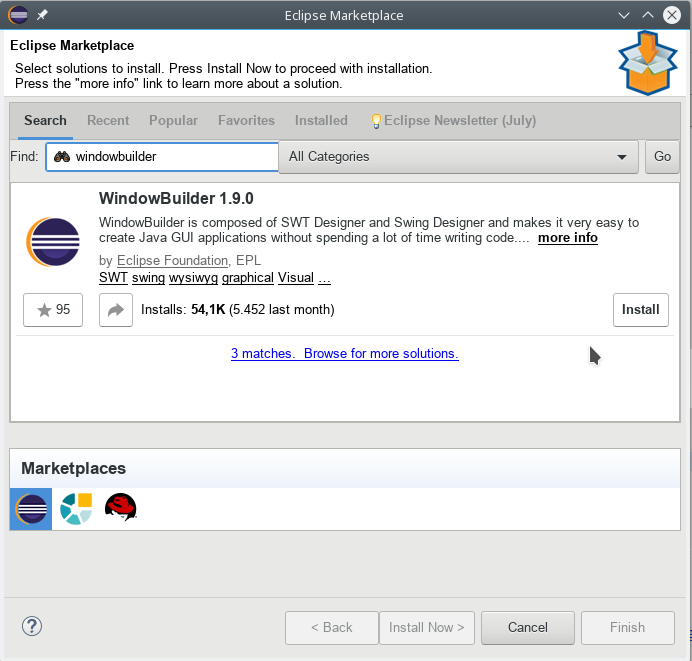
\includegraphics[width=0.6\textwidth]{./inf/SEKII/01_Vorbereitung/windowbuilder_plugin.png}
   \caption{WindowBuilder Plugin installieren}
   \label{fig:windowbuilder-plugin}
\end{figure}

$\rightarrow$ \myPMI{Confirm} $\rightarrow$ Häkchen setzen vor
\myPMI{Accept Licence Agreement} $\rightarrow$ \myPMI{Finish} $\rightarrow$
\myPMI{Restart Now}


\subsection{Installation des
MySQL-Java-Connectors}\label{mysql-connector-installation}

Zunächst musst du den Connector herunter laden:

\url{https://www.dropbox.com/s/rozd9ovbnti4rkl/mysql-connector-java-8.0.18.jar?dl=0}

(Sobald wir im Unterricht bei SQL angekommen sind, wirst du diese Datei auch in
unserem Kurs-Repository finden. Und bis dahin brauchst du dich um die
Einbindung des Connectors auch noch nicht zu kümmern.)

Rechtsklick auf dein Projekt $\rightarrow$ \myPMI{Import \ldots} $\rightarrow$
\myPMI{General} $\rightarrow$ \myPMI{File System} $\rightarrow$ \myPMI{Next}
$\rightarrow$ \myPMI{From directory:} (\myPMI{Browse} -- dort das Verzeichnis
wählen, in dem die JAR-Datei des Connectors liegt) $\rightarrow$ \myPMI{Next}
$\rightarrow$ im folgenden Dialog die gewünschte Datei auswählen $\rightarrow$
\myPMI{Finish}.

Rechtsklick auf deinen Projekt-Ordner im Package-Explorer $\rightarrow$
\myPMI{Build Path} $\rightarrow$ \myPMI{Configure Build Path \ldots}
$\rightarrow$ Wähle den Reiter \myPMI{Libraries} $\rightarrow$ \myPMI{Add JARs
\ldots} $\rightarrow$ wähle \myFile{mysql-connector-java-8.0.18.jar} in
deinem Projekt $\rightarrow$ \myPMI{OK} $\rightarrow$ \myPMI{OK}.

\subsection{Installation des DBeaver Plugins}

Analog zur Installation des WindowsBuilder Plugins werden wir in Q2 auch noch 
das DBeaver Plugin installieren müssen.

\myPMI{Help} $\rightarrow$ \myPMI{Eclipse Marketplace\ldots}

Im Suchfeld gibst du \myPMI{DBeaver} ein und lässt den Marktplatz
durchsuchen (siehe Abbildung \ref{fig:dbeaver-plugin}).

\begin{figure}[h]
  \centering
   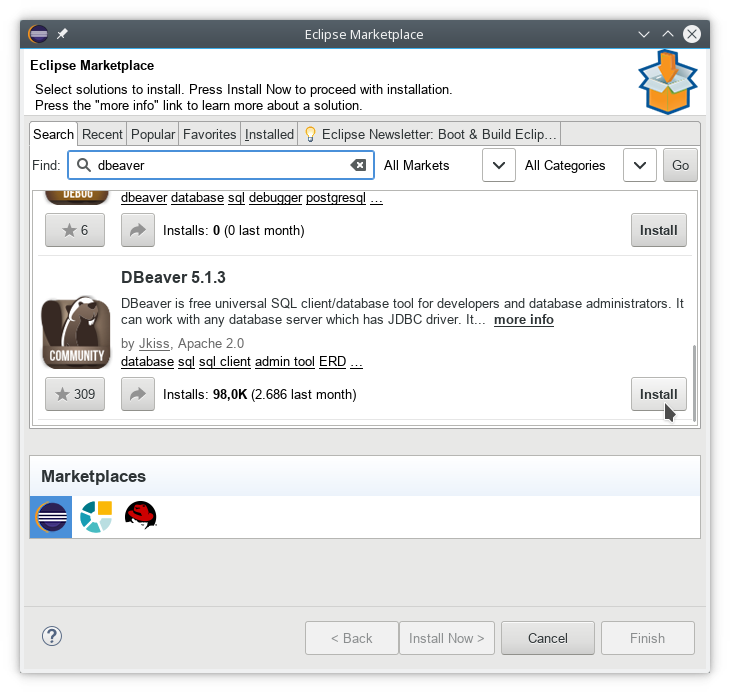
\includegraphics[width=0.6\textwidth]{./inf/SEKII/01_Vorbereitung/dbeaver_plugin.png}
   \caption{DBeaver Plugin installieren}
   \label{fig:dbeaver-plugin}
\end{figure}

Nun kannst du das DBeaver Plugin installieren lassen:

$\rightarrow$ \myPMI{Confirm} $\rightarrow$ Häkchen setzen vor
\myPMI{Accept Licence Agreement} $\rightarrow$ \myPMI{Finish} $\rightarrow$
\myPMI{Restart Now}

Nach erfolgter Installation des Plugins und anschließendem Neustart von Eclipse,
fügst du mit \myPMI{Window} $\rightarrow$ \myPMI{Show View} $\rightarrow$
\myPMI{Other \ldots} $\rightarrow$ \myPMI{Database} $\rightarrow$ 
\myPMI{Database Navigator} $\rightarrow$ \myPMI{Open} den Database Navigator View 
hinzu (er wird als zusätzlicher Tab unten in Eclipse angezeigt).

Dort kannst du -- einen laufenden MySQL- oder MariaDB-Server vorausgesetzt -- die
Verbindung (Connection) zum Datenbankserver konfigurieren:

Rechtsklick im Database Navigator View $\rightarrow$ \myPMI{Create New Connection}. 
Aus der nun angebotenen langen Liste wähltst du \myPMI{MySQL 8.x} aus und bestätigst 
mit \myPMI{Next}. Im folgenden Dialog gibst du für \myPMI{Username} und 
\myPMI{Passwort} jeweils \myUserInput{root} ein.

Als \myPMI{Server Time Zone} wähltst du im selben Dialog \myUserInput{Europe/Berlin}
aus (siehe Abbildung \ref{fig:dbeaver_connection_settings}).

\begin{figure}[h]
  \centering
   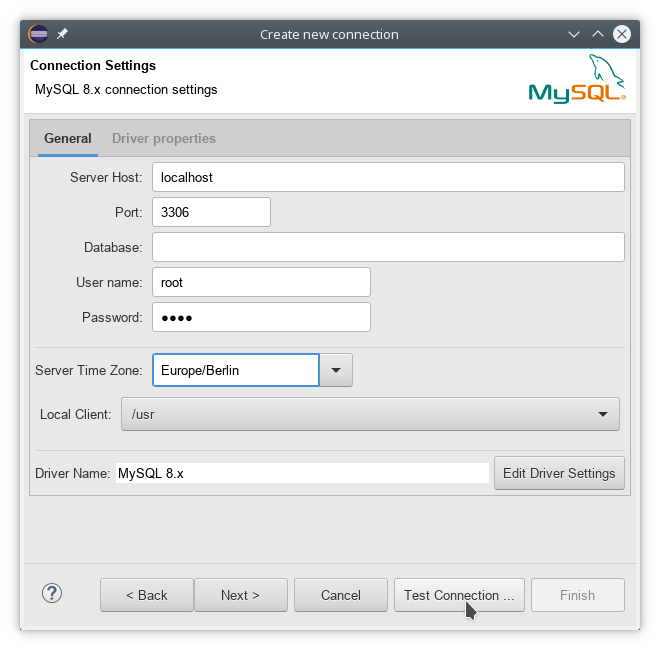
\includegraphics[width=0.6\textwidth]{./inf/SEKII/01_Vorbereitung/dbeaver_connection_settings.png}
   \caption{Verbindung zum Datenbankserver konfigurieren}
   \label{fig:dbeaver_connection_settings}
\end{figure}

Als nächstes wähltst du \myPMI{Test Connection \ldots} aus: Eclipse (bzw.\ das DBeaver 
Plugin) wird nun erkennen, dass ein Treiber für die Verbindung zum Datenbankserver
fehlt. Ein entsprechender Download wird automatisch angeboten und von dir akzeptiert
(Button \myPMI{Download}). Siehe Abbildung \ref{fig:dbeaver_download_driver}.

\begin{figure}[h]
  \centering
   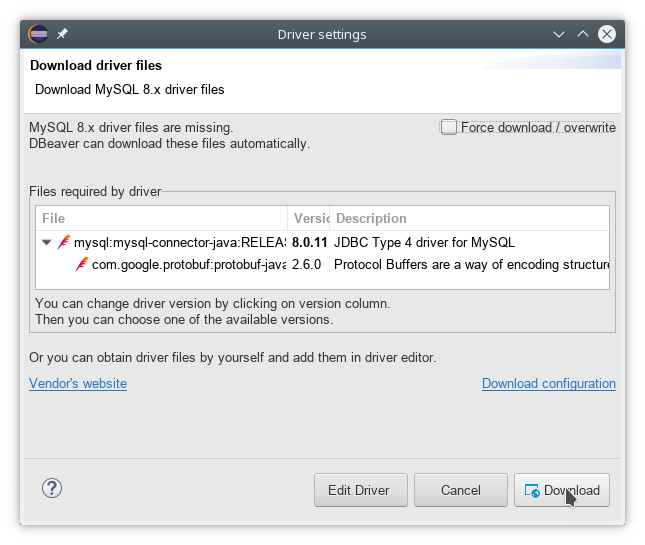
\includegraphics[width=0.6\textwidth]{./inf/SEKII/01_Vorbereitung/dbeaver_download_driver.png}
   \caption{Treiber für die Verbindung zum Datenbankserver installieren lassen}
   \label{fig:dbeaver_download_driver}
\end{figure}

Falls der Datenbankserver bereits installiert wurde und aktuell auch läuft, sollte 
direkt im Anschluss an den Download des Treibers eine Erfolgsmeldung zum Test der 
Verbindung zum Datenbankserver ausgegeben werden.

Abschließend verlässt du den New Connection Dialog mit \myPMI{Next} $\rightarrow$ 
\myPMI{Next} $\rightarrow$ \myPMI{Finish} ohne an den weiteren Einstellungen etwas zu 
verändern.

Die Verbindung zum lokalen Datenbankserver ist nun konfiguriert. Aktiviert wird sie
über einen Rechtsklick auf den neuen Eintrag im Database Navigator View $\rightarrow$ 
\myPMI{Connect}. Ein kleiner Haken vor dem Eintrag im Database Navigator View zeigt
die bestehende Verbindung an.

Ab sofort kannst du in Eclipse auch SQL Dateien bearbeiten: Entweder vorhandene Dateien 
öffnen oder mit \myPMI{File} $\rightarrow$ \myPMI{New} $\rightarrow$
\myPMI{Other \ldots} $\rightarrow$ \myPMI{General} $\rightarrow$ 
\myPMI{File} eine neue Datei mit Dateiendung \myUserInput{*.sql} erstellen.
Solche Dateien werden nun automatisch mit dem SQL Editor geöffnet.

% \subsection{Plugin „SQL-Explorer“ installieren und konfigurieren}
% 
% \myPMI{Help} $\rightarrow$ \myPMI{Install New Software \ldots} $\rightarrow$
% \myPMI{Add} $\rightarrow$ bei Name: \myUserInput{SQL-Explorer} und bei Location:
% 
% \url{http://eclipsesql.sourceforge.net/} 
% 
% eintragen. Mit \myPMI{OK} bestätigen. Wenn man den nun sichtbaren Eintrag für
% \myPMI{SQL Explorer} auffaltet, sieht man möglicherweise mehrere Versionen des
% Plugins. Davon die aktuellste auwählen. Mit \myPMI{Next} bestätigen. Nochmals
% \myPMI{Next}. Dann \myPMI{I accept the terms of the license agreement}
% $\rightarrow$ \myPMI{Finish}. Die im Installationsverlauf erscheinende Warnung
% bezüglich der Installation nicht-signierter Inhalte mit \myPMI{OK} quittieren.
% Ebenso den Hinweis auf den nötigen Neustart von Eclipse.
% 
% Anschließend muss noch die Verbindung zum lokalen MySQL-Server konfiguriert
% werden:
% 
% \myPMI{Windows} $\rightarrow$ \myPMI{Show View} $\rightarrow$ \myPMI{Other
% \ldots} $\rightarrow$ \myPMI{SQL Explorer} $\rightarrow$ \myPMI{Connections}
% $\rightarrow$ \myPMI{OK} Im nun verfügbaren Connections-Tab (unten)
% $\rightarrow$ Rechtsklick $\rightarrow$ \myPMI{New Connection Profile \ldots}
% $\rightarrow$ Name: \myUserInput{MySQL localhost} $\rightarrow$ \myPMI{Add/Edit
% Drivers} $\rightarrow$ \myPMI{SQL Explorer} auffalten $\rightarrow$ \myPMI{JDBC
% Drivers} $\rightarrow$ Doppelklick auf  \myPMI{MySQL Driver} $\rightarrow$
% \myPMI{Extra Class Path} $\rightarrow$ \myPMI{Add JARs \ldots} $\rightarrow$
% Den Pfad zu \myFile{mysql-connector-java-8.0.12.jar} (oder neuere Version)
% auf der lokalen Platte (vermutlich in einem Unter-Ordner des workspace-Ordners)
% auswählen.
% 
% Siehe Abbildung \ref{fig:mysql-connector}.
% 
% \begin{figure}[h]
%   \centering
%    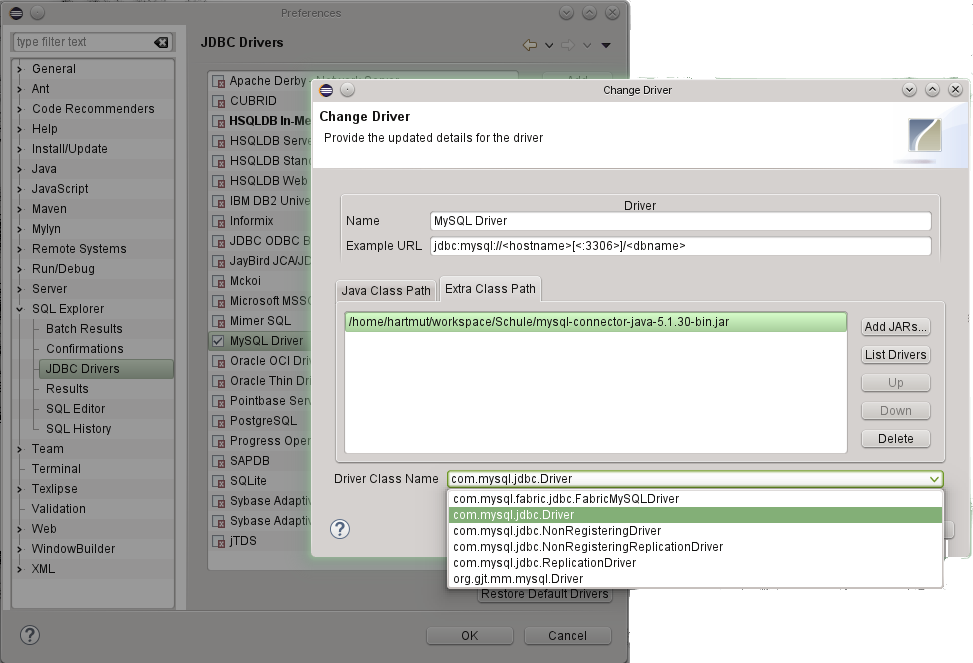
\includegraphics[width=1.0\textwidth]{./inf/SEKII/01_Vorbereitung/MySQL-Driver.png}
%    \caption{Auswahl des MySQL-Connectors}
%    \label{fig:mysql-connector}
% \end{figure}
% 
% $\rightarrow$ \myPMI{List Drivers} $\rightarrow$ aus der
% Dropdown-Liste für \myPMI{Driver Class Name} den Eintrag
% \myUserInput{com.mysql.jdbc.Driver} auswählen $\rightarrow$ \myPMI{OK}
% $\rightarrow$ \myPMI{OK} $\rightarrow$ Driver: \myPMI{MySQL Driver}
% $\rightarrow$ Häkchen Setzen bei \myPMI{Auto Logon} und \myPMI{Auto Commit}
% $\rightarrow$ Anpassen der URL auf \myUserInput{jdbc:mysql://localhost:3306/}
% $\rightarrow$ \myPMI{User:} „root“ $\rightarrow$ \myPMI{Password:} „root“
% $\rightarrow$\myPMI{OK}.
% 
% Siehe Abbildung \ref{fig:sql-explorer-connection-profile}.
% 
% \begin{figure}[h]
%   \centering
%    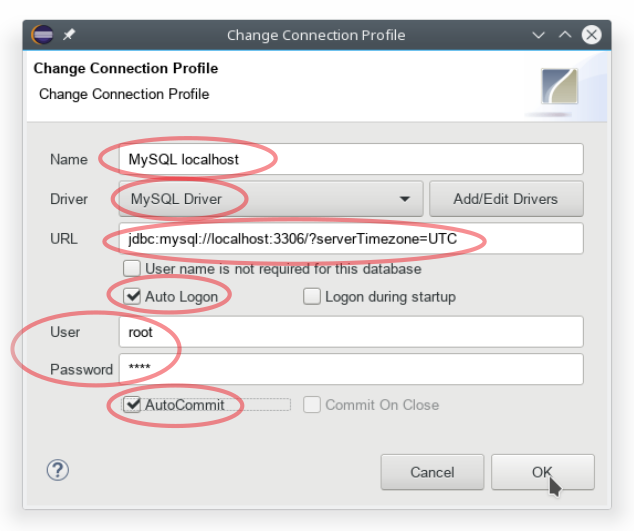
\includegraphics[width=0.7\textwidth]{./inf/SEKII/01_Vorbereitung/SQL-Explorer_Connection-Profile.png}
%    \caption{Einstellungsdialog für die Verbindung zum lokalen MySQL-Server}
%    \label{fig:sql-explorer-connection-profile}
% \end{figure}
% 
% Ab sofort werden SQL-Skripte in Eclipse mit dem SQL-Explorer geöffnet. In diesem
% kann (einen lokal laufenden MySQL-Server vorausgesetzt)  dann einfach eine
% Verbindung zum lokalen MySQL-Server hergestellt werden. Im Drop-Down-Menü,
% links von \myPMI{Limit Rows} in der Menüzeile des SQL-Explorer Fensters kann
% dazu einfach der Eintrag \myPMI{MySQL localhost/root} ausgewählt werden.



\section{Eclipse kennen lernen}

Für die ersten Schritte in Eclipse empfehle ich dir Video-Tutorials zu Java mit Eclipse.
Beispielsweise auch eine ganze Serie (von brauchbarer Qualität):

\url{http://www.youtube.com/playlist?list=PL71C6DFDDF73835C2}
